\chapterimage{Mavrica.jpg} % Chapter heading image

\chapter{Koherenca}

V tem poglavju bomo spoznali \index{Koherenca}koherenco. To je lastnost
valovanja, ki je tesno povezana s pojavom interference. Ohlapno pravimo,
da je koherentno tisto valovanje, s katerim se posrečijo interferenčni
poskusi.  

\section{Youngov poskus}

\index{Interferenca}Interferenčnih pojavov ni mogoče opazovati z
vsakim svetlobnim izvorom. Da bi to razumeli, si oglejmo interferenco
valovanja, ki vpada na dve majhni reži (tako imenovani \index{Youngov poskus}Youngov 
poskus\footnote{Angleški znanstvenik Thomas Young, 1773--1829.}). 
Navadno predpostavimo, da
sta obe reži osvetljeni z istim ravnim valom. Delni valovanji, ki
izhajata iz rež, imata tako ves čas poskusa enako polarizacijo, enako
frekvenco in enako fazno razliko. Zaradi različnih dolžin poti obeh
delnih valovanj od reže do dane točke na zaslonu dobimo na oddaljenem
zaslonu interferenčni vzorec (slika~\ref{fig:Young}). Vendar dobimo 
interferenco le v primeru,
ko je faza valovanja, ki vpada na reži, konstantna. Svetloba s konstantno
fazo je koherentna in jo dobimo, na primer, iz kvalitetnega laserja.
Svetloba iz običajnih svetil ne da interferenčnega vzorca, zato zanjo
pravimo, da ni koherentna. 
\begin{figure}[h]
\centering
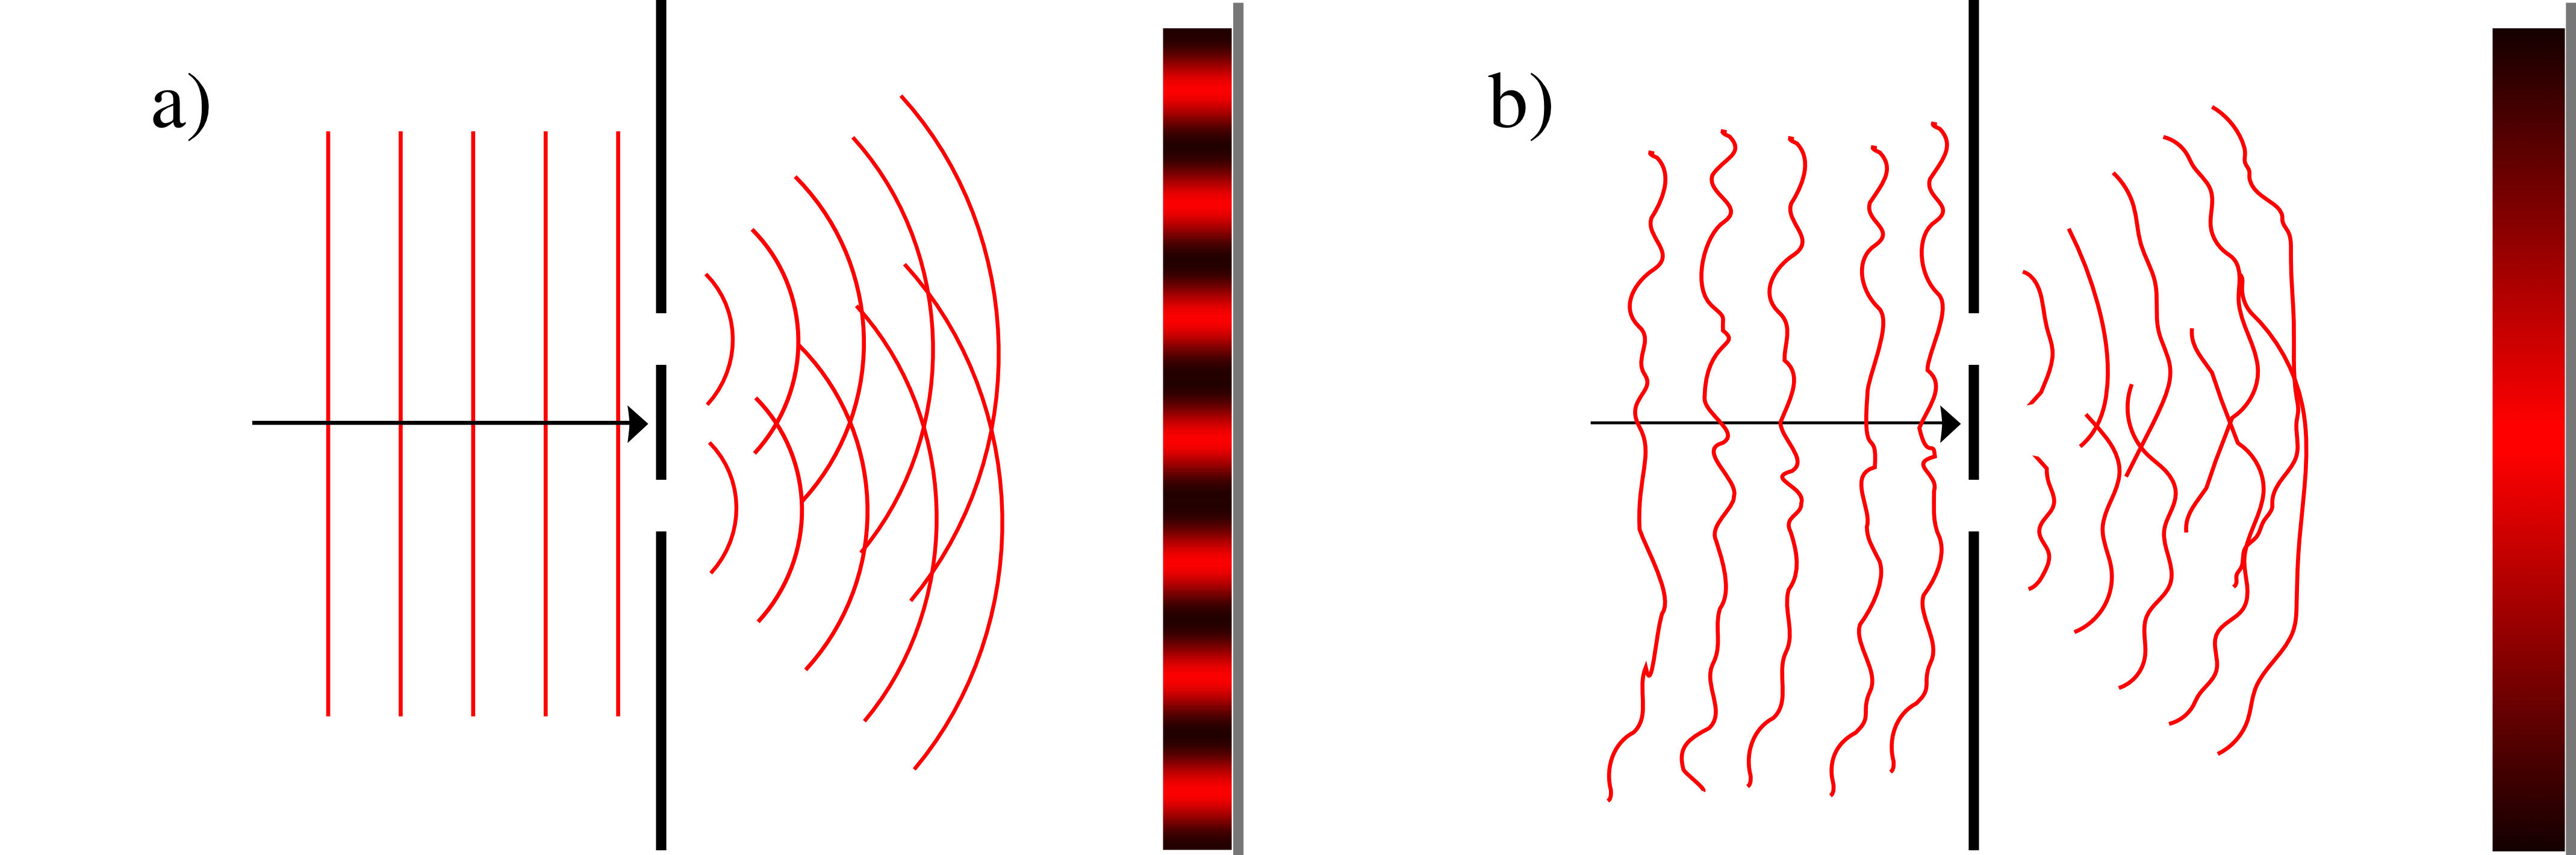
\includegraphics[width=11truecm]{slike/02_Young.png}
\caption{Youngov poskus na dveh režah. Le če je vpadno valovanje koherentno, dobimo
na zaslonu interferenčni vzorec.}
\label{fig:Young}
\end{figure}

\noindent
Svetloba običajnih svetil, na primer plinskih razelektritvenih cevi
(sijalk), je zaradi vrste nastanka kaotične narave. 
Atomi sevajo neodvisno, zato se faza izsevanega valovanja
spreminja. Približno konstantna je le znotraj nekega karakterističnega
časa. Če je pri interferenčnem poskusu karakteristični čas spreminjanja
faze manjši od zakasnitve med valovanjema, ki nastane zaradi različno
dolgih poti, dobimo na danem mestu zaslona zdaj konstruktivno, zdaj
destruktivno interferenco. Ker je ta čas praviloma
bistveno krajši od časa, v katerem opazujemo interferenco,
utripanje svetlobe na zaslonu ni vidno. Interferenčni poskus se ni 
posrečil zaradi majhne časovne koherence\index{Časovna koherenca},
karakterističnemu času spreminjanja faze pa rečemo \index{Koherenčni čas}koherenčni čas
$t_{c}$. Časovno koherenco bomo natančneje obravnavali v razdelku
(\ref{sec:casovna-koherenca}), zaenkrat povejmo le, da je časovna
koherenca vezana na fazno razliko med dvema točkama, ki ležita
vzdolž smeri širjenja valovanja. \\

\noindent
Poleg časovne koherence na interferenčno sliko pomembno vpliva tudi
\index{Prostorska koherenca}prostorska koherenca, ki je posledica
končne dimenzije svetila. Svetloba, ki vpada na reži z različnih delov
svetila, ima namreč različno fazo zaradi različnih dolžin poti od
svetila do rež. Ta faza se prišteje fazni razliki zaradi različno
dolgih poti od rež do zaslona, zaradi česar se na zaslonu interferenčne
proge nekoliko premaknejo. Če je fazna razlika žarkov iz različnih
delov svetila večja od fazne razlike za režami, se celotna interferenčna
slika na zaslonu izpovpreči. Interferenco pri Youngovem poskusu
dobimo, kadar sta reži razmaknjeni le toliko, da je povprečna fazna
razlika manjša od $2\pi$. Največjemu prečnemu razmiku, ki še da interferenco,
rečemo prečna koherenčna razdalja\index{Koherenčna razdalja} $d_{c}$. Prostorska koherenca,
ki jo bomo podrobneje spoznali v razdelku (\ref{Prostorska-koherenca}),
je torej vezana na fazno razliko med dvema točkama, ki ležita prečno 
na smer širjenja valovanja.\\

\noindent
Poudarimo še enkrat, da je pojem koherence statističen.
Če je koherenčni čas $t_{c}$ dolg v primerjavi s časom opazovanja,
se vedno seštevajo amplitude valovanj in dobimo interferenčno sliko.
Ta se slučajno spreminja z značilnim časom $t_{c}$. Če pa so razlike
poti večje od $ct_{c}$ ali razmik rež večji od $d_{c}$, gledamo
le povprečno sliko in interferenčne proge izginejo.

\section{Koherenca običajnih svetil}

Vzemimo za izvor plinsko razelektritveno cev in z
ustreznim filtrom izberimo eno samo spektralno črto. Ta črta naj ima
osrednjo frekvenco $\nu_{0}$ in končno frekvenčno širino $\delta\nu$,
ki je kombinacija naravne širine, razširitve zaradi trkov med atomi
in zaradi Dopplerjevega pojava (glej poglavje ***). Privzemimo,
da je glavni prispevek k razširitvi spektralne črte zaradi med\-atomskih
trkov, razširitev, povezano z Dopplerjevim efektom, pa zanemarimo.\\

\noindent
Celotna izsevana svetloba je vsota delnih valov, ki izhajajo iz posameznih
atomov in so zato med seboj neodvisni. Vsak delni val ohranja konstantno
fazo med dvema trkoma, to je v časovnem intervalu $t_{c}$. Valovni
paket dolžine $t_{c}$ mora vsebovati frekvence v pasu $\Delta\omega$,
za katerega velja $t_{c}\Delta\omega\sim1$. Koherenčni čas je torej
kar reda velikosti obratne vrednosti spektralne širine svetlobe. Povsem
monokromatsko valovanje bil imelo neskončen koherenčni čas in bi bilo
popolno koherentno.\\

\noindent
Zapišimo še izsevano polje takega svetila. 
Jakost električnega polja v izbrani točki prostora je vsota delnih
valov, ki izvirajo iz raznih delov izvora. Vsak atom v izvoru, naj
jih bo $N$, seva neodvisno, zato so tudi delna valovanja med seboj
neodvisna. Posamična valovanja ohranjajo konstantno fazo v času med
dvema trkoma atoma, $t_{c}$. Zaradi enostavnosti privzemimo,
da so amplitude $E_{1}$ in polarizacije izsevanih polj posameznih atomov enake. 
Električno poljsko jakost $E$ v izbrani točki prostora lahko 
zapišemo kot vsoto posameznih prispevkov
\begin{equation}
E=E_{1}\sum_{n=1}^{N}e^{i\phi_{n}(t)}.
\label{eq:amplituda-random}
\end{equation}
kjer se faza polja $\phi_{n}(t)$, ki ga izseva posamezni atom, naključno
spremeni ob trku z drugim atomom. Povprečna velikost
vsote polj $E$ je nič, povprečni kvadrat skupnega polja, ki je sorazmeren
z gostoto svetlobnega toka, pa je $NE_{1}^{2}$. Zaradi slučajnosti faz je 
slučajna tudi faza celotnega polja in se gotovo povsem spremeni v času, ko se
spremeni faza posameznih prispevkov, to je $t_{c}$. S tako svetlobo bomo videli 
interferenco na režah, če bo razlika poti delnih valovanj manjša od $c\, t_{c}$.\\

\noindent
Oglejmo si izračun
na primeru. Imejmo $N=100$ neodvisnih atomov, ki se jim faza naključno
spreminja s karakterističnim časom $t_{c}=10/\nu$, kjer je $\nu$
frekvenca valovanja. Na sliki (\ref{fig:amplituda-intenziteta}) sta
prikazana časovna poteka amplitude $E$ (enačba \ref{eq:amplituda-random})
in $|E|^{2}$, ki je sorazmeren z intenziteto svetlobe.
\begin{figure}
\centering
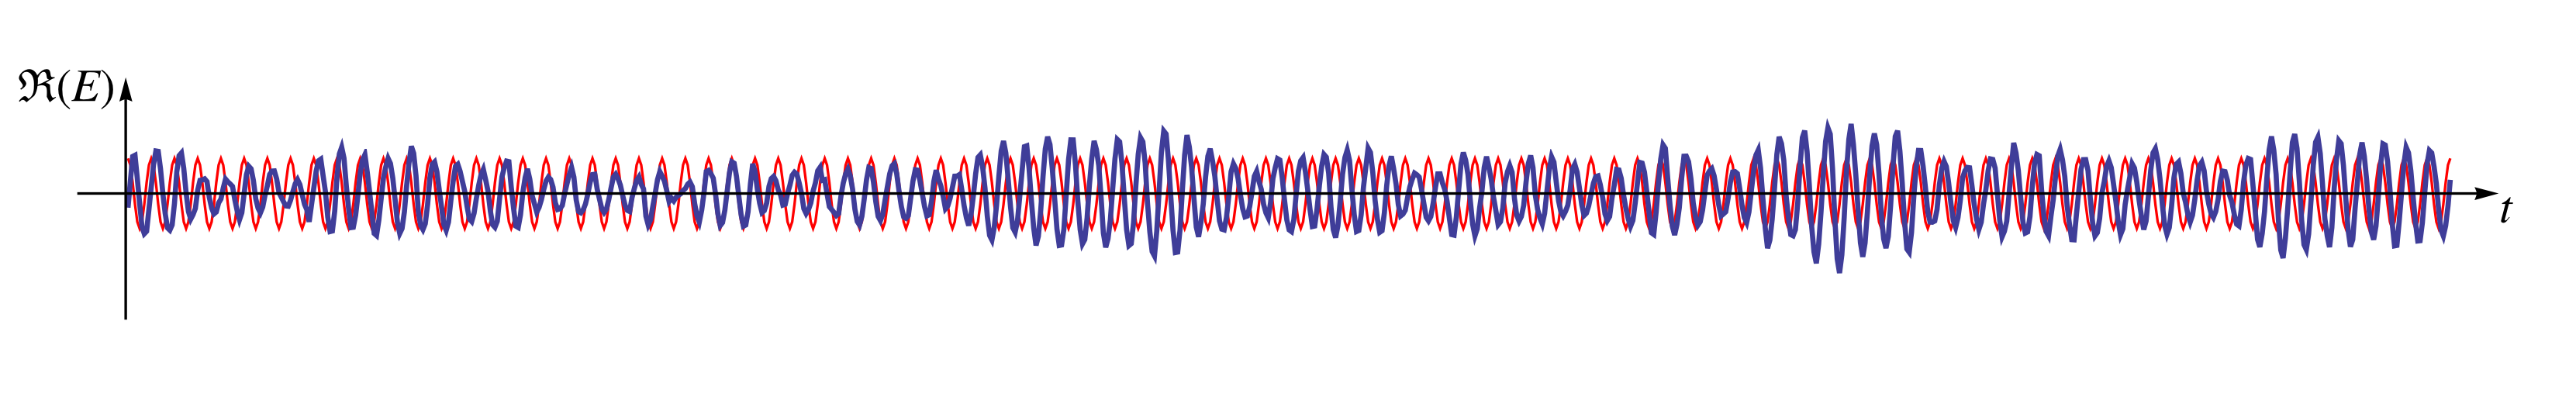
\includegraphics[width=15truecm]{slike/02_fluktuacije.png}\\
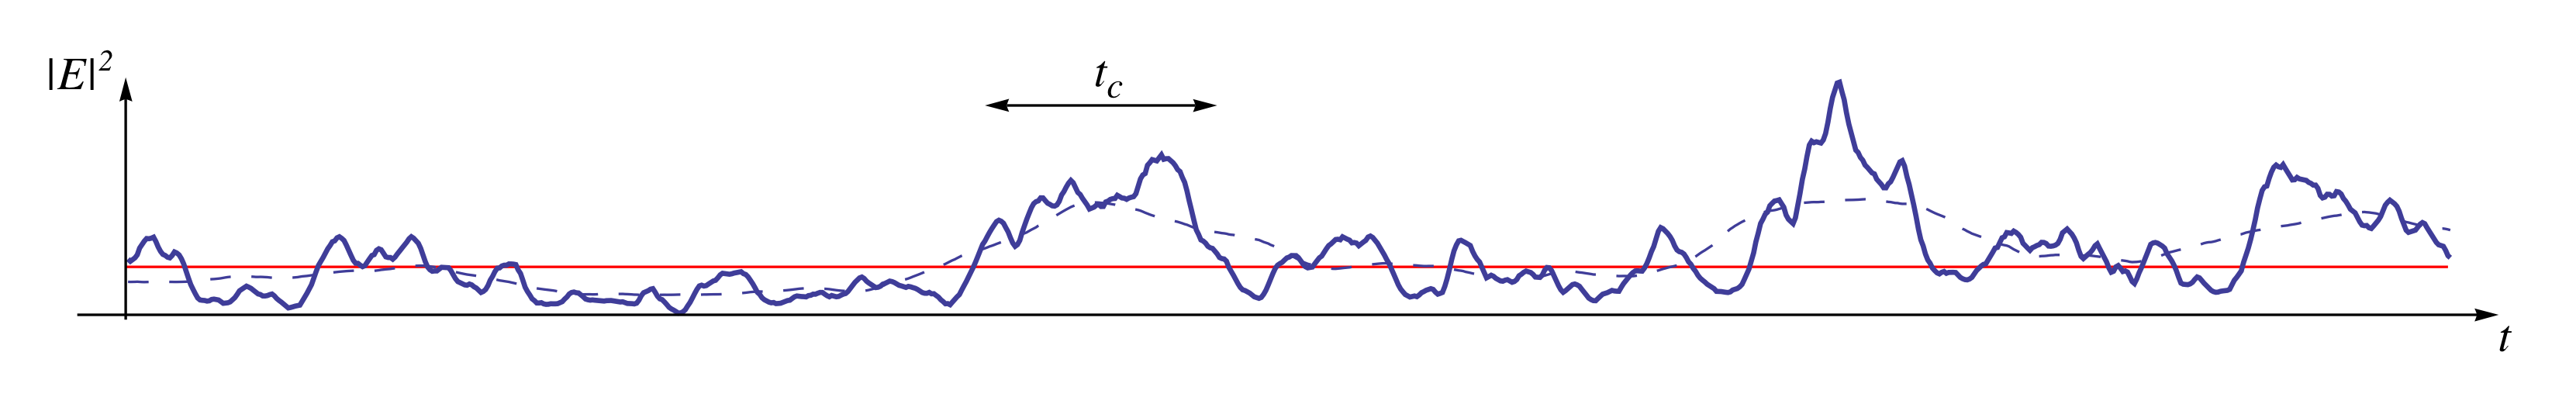
\includegraphics[width=15truecm]{slike/02_fluktuacije2.png}
\caption{Zgoraj: shematski prikaz električne poljske jakosti 
ravnega vala s konstantno fazo (rdeča črta) in električne
poljske jakosti običajnega svetila (modra črta) kot funkcije
časa. Faza polja se naključno spreminja s karakterističnim časom $t_{c}$.
Spodaj: intenziteta ravnega vala (rdeča črta) in intenziteta
svetlobe običajnega svetila (modra črta) kot funkcije
časa. Modra črtkana črta je povprečna intenziteta 
$\frac{1}{T}\int_{-T/2}^{T/2}E(t+t')E^{*}(t+t')dt'$
s časom integracije $T=t_{c}$. }
\label{fig:amplituda-intenziteta}
\end{figure}
Za primerjavo je prikazan tudi ravni val $E=\sqrt{N}E_{1}e^{-i\omega t}$
s konstantno fazo in njegova intenziteta. Intenziteta ravnega vala je konstantna, 
medtem ko je povprečna intenziteta svetlobe običajnega svetila približno 
konstantna le znotraj $t_{c}$.\\

\section{Časovna koherenca}
\label{sec:casovna-koherenca}

Časovno koherenco\index{Časovna koherenca} je najlažje obravnavati 
z \index{Michelsonov interferometer}Michelsonovim 
interferometrom\footnote{Ameriški fizik in nobelovec Albert Abraham Michelson, 1852--1931.},
ki je prikazan na sliki (\ref{fig:michelson}). Valovanje iz točke $P$ na polprepustnem 
zrcalu razdelimo na dva delna snopa, nato enega s premikanjem zrcala zakasnimo za $\tau=2x/c$.
S kolimacijsko lečo dosežemo, da je čim več žarkov, ki izhajajo iz
$P$, vzporednih z osjo interferometra. Dokler je zakasnitev
$\tau$ manjša od koherenčnega časa $t_{c}$,
dobimo na detektorju interferenčne vrhove in doline. Pri zakasnitvah,
ki so večje od koherenčnega časa, ni stalne fazne povezave, interferenčna
slika se spreminja in v daljših časih izpovpreči. Zapišimo to ugotovitev
še matematično.
\begin{figure}[h]
\centering
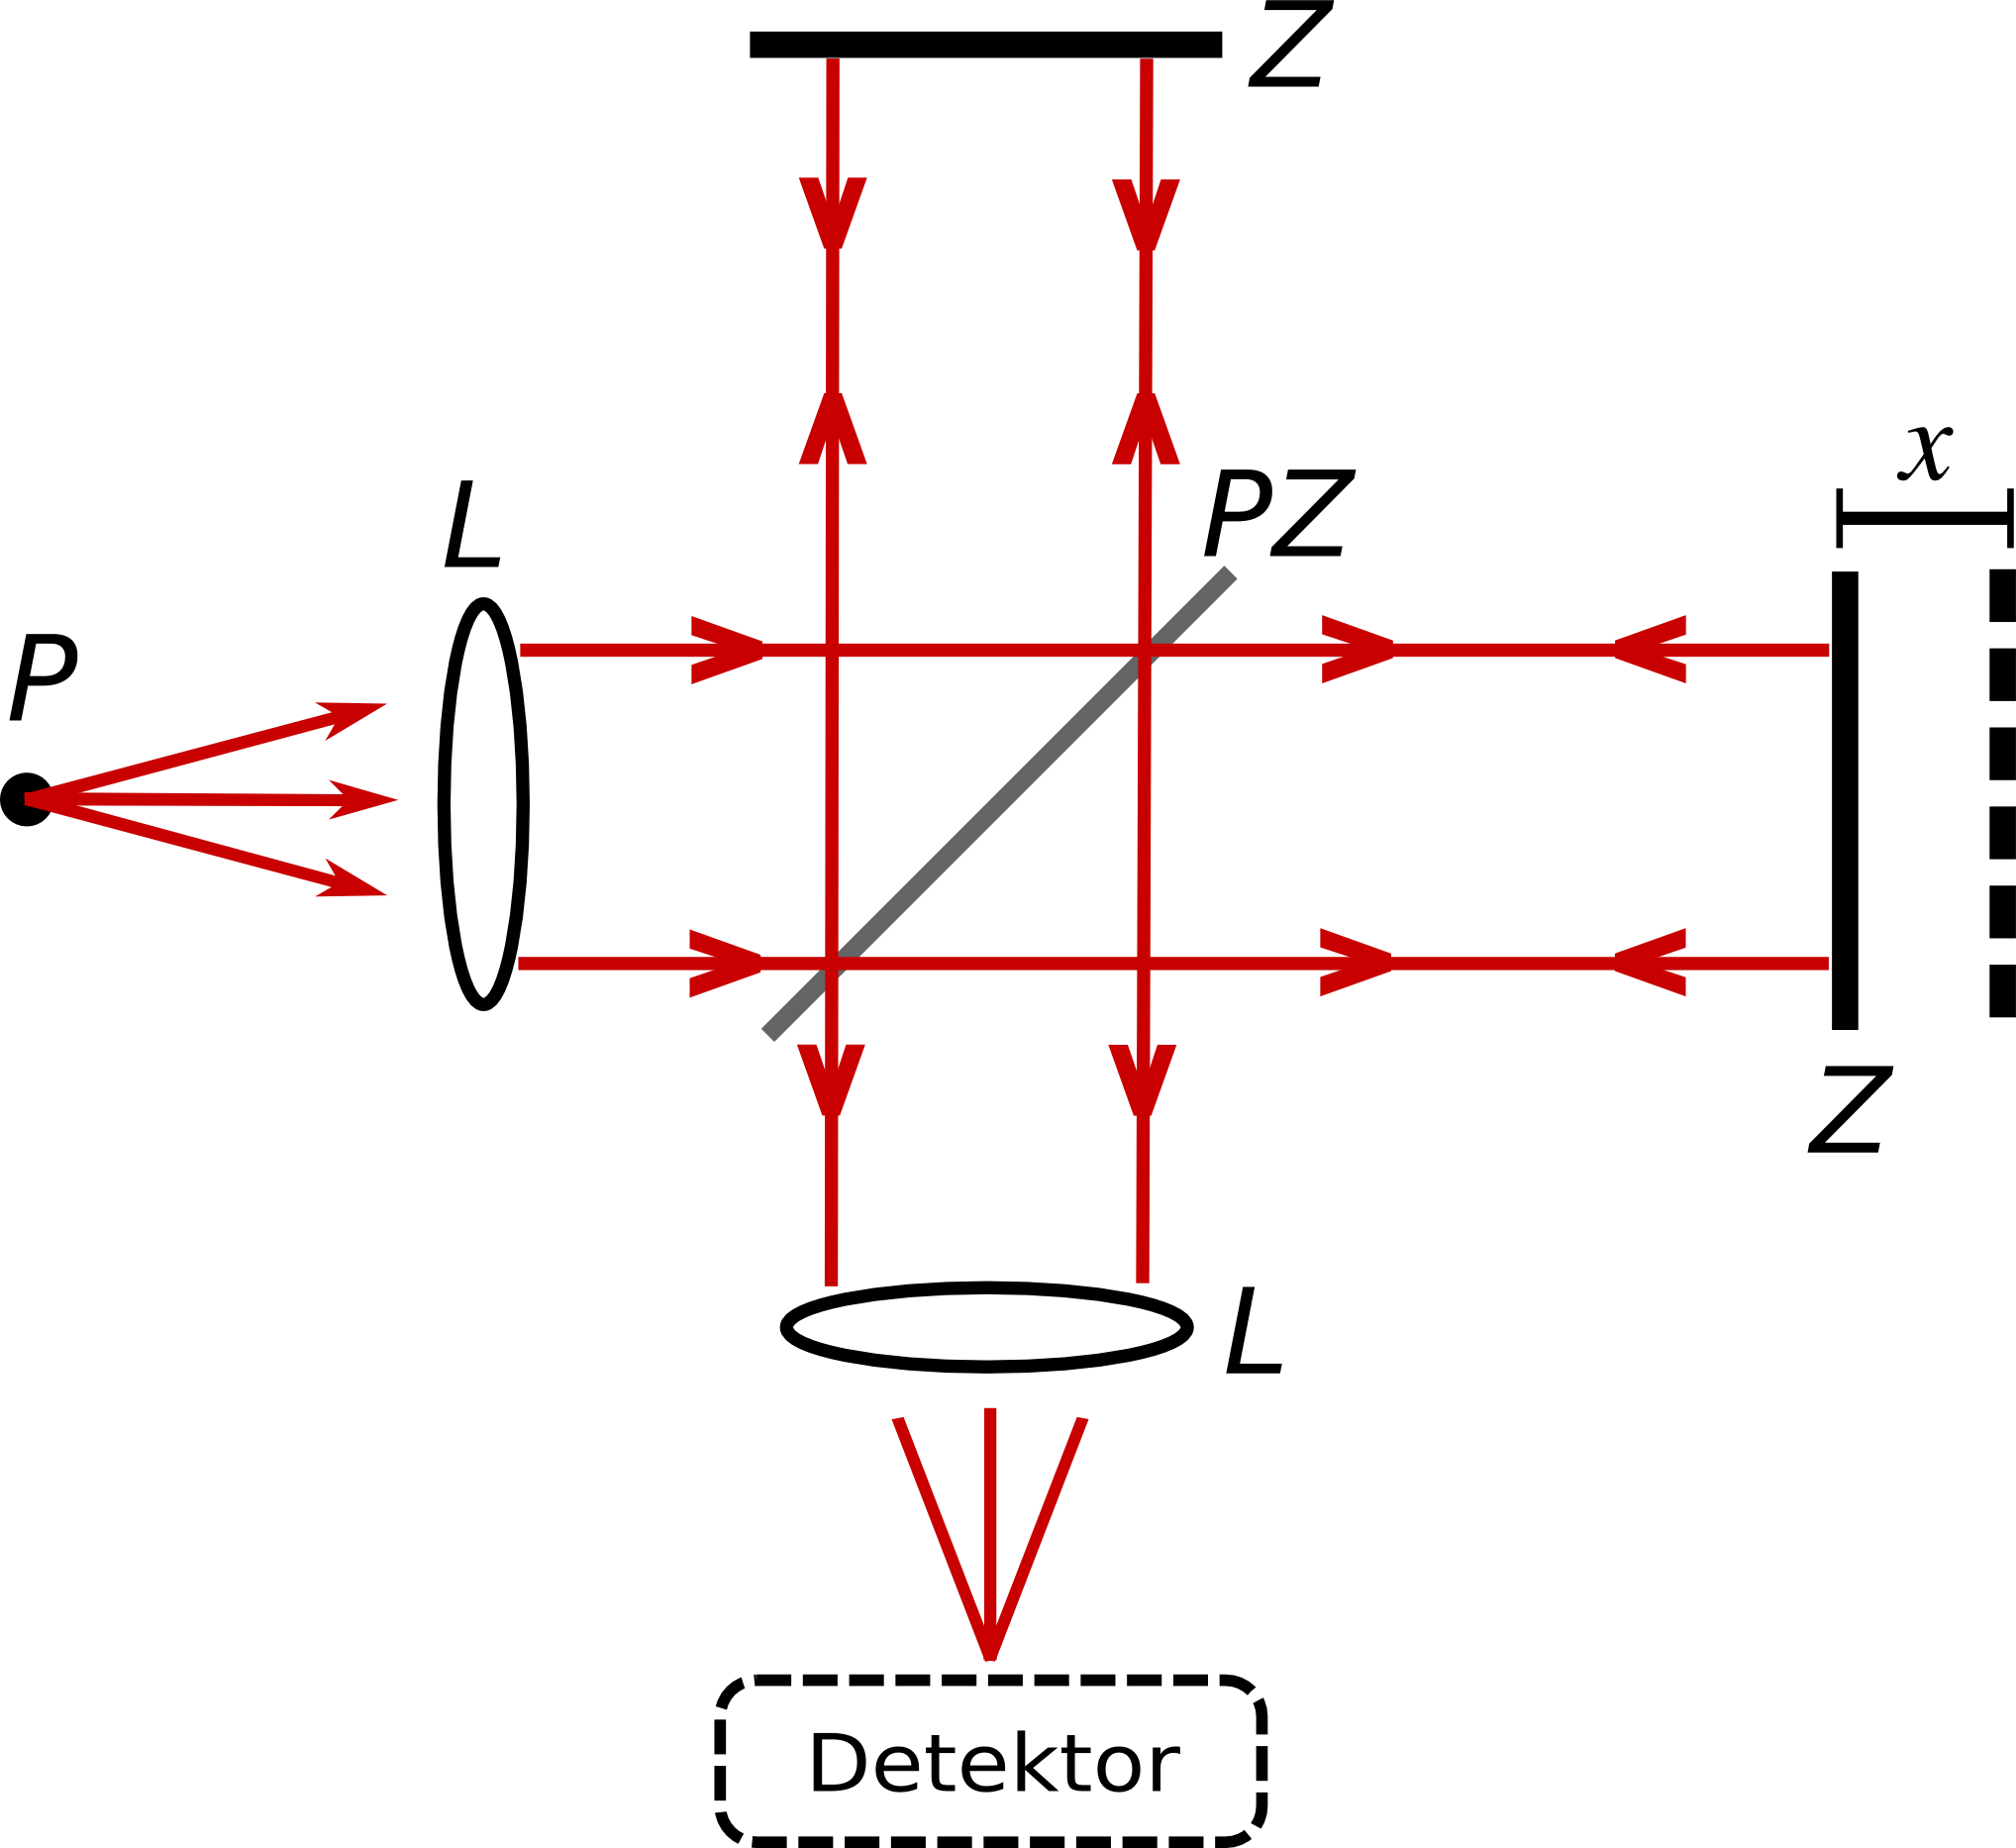
\includegraphics[width=6truecm]{slike/02_Michelson.png}
\caption{\label{fig:michelson}Michelsonov interferometer. Svetlobo
iz izvora $P$ usmerimo preko kolimacijske leče ($L$) na polprepustno
zrcalo ($PZ$), s čimer jo razdelimo na dva snopa. S premikom
enega zrcala ($Z$) en delni žarek zakasnimo. Interferenco opazujemo na detektorju.}
\end{figure}

\noindent
Svetlobni tok na detektorju je sorazmeren s kvadratom električne
poljske jakosti obeh delnih valovanj
\begin{equation}
|E_{d}(t)|^{2}=|E(t)+E(t+\tau)|^{2}=|E(t)|^{2}+|E(t+\tau)|^{2}+2\Re E(t)E^{*}(t+\tau).
\label{eq:Michelson-intenziteta}
\end{equation}
Zakasnitev $\tau$ je določena s premikom pomičnega zrcala, $\tau=2x/c$.
Navadno opazujemo v času $T$, ki je dolg v primerjavi s koherenčnim
časom, zato povprečimo po času
\begin{eqnarray}
\langle|E_{d}|^{2}\rangle & = & \frac{1}{T}\int_{-T/2}^{T/2}|E{}_{d}(t)|^{2}\, dt\nonumber \\
 & = & 2\langle|E|^{2}\rangle+2\Re\langle E(0)E^{*}(\tau)\rangle = 2\langle|E|^{2}\rangle+2\Re G(\tau).
\end{eqnarray}
Prvi člen je vsota povprečnih svetlobnih tokov obeh delnih snopov. Privzeli
smo, da je polje v povprečju stacionarno in je zato povprečje neodvisno
od izbire časovnega intervala. Drugi člen opisuje interferenco. Pri tem smo vpeljali
časovno avtokorelacijsko funkcijo\index{Avtokorelacijska funkcija}
električnega polja 
\boxeq{eq:avtokorelacija}{
G(\tau)=\frac{1}{T}\int_{-T/2}^{T/2}E(t)E^{*}(t+\tau)\, dt.
}
Za majhne zakasnitve $\tau$ je $|G(\tau)|\approx|G(0)|=1$ in na
detektorju zaznamo interferenco. Za zakasnitve $\tau,$ ki so precej
večje od koherenčnega časa $t_{c}$, sta polji $E(0)$ in $E(\tau)$
statistično neodvisni in povprečje produkta je enako produktu povprečij.
Ker je $\langle E(t)\rangle=0$, pri velikih zakasnitvah $\tau$ interferenčni
člen izgine in svetlobni tok je enak vsoti tokov posameznih delnih
snopov. \\

\noindent
Priročno je vpeljati normirano avtokorelacijsko funkcijo 
\begin{equation}
g(\tau)=\frac{G(\tau)}{G(0)}.
\label{eq:avtokorelacija-norm}
\end{equation}
Za povsem koherentno valovanje je $|g(\tau)|=1$, za povsem nekoherentno
valovanje je $|g(\tau)|=0,$ za delno koherentna  pa $0<|g(\tau)|<1$.
Praviloma se vrednost $|g(\tau)|$ z naraščajočim $\tau$ zmanjšuje,
saj postaja valovanje za velike časovne zamike vedno manj korelirano.
Ohlapno povedano je koherenčni čas zakasnitev, pri kateri postane
vrednost avtokorelacijske funkcije majhna.
Koherenčni čas\index{Koherenčni čas} $t_{c}$ pa lahko tudi bolj natančno definiramo 
z normirano avtokorelacijsko funkcijo: 
\begin{equation}
t_{c}=\int_{-\infty}^{\infty}\left|g(\tau)\right|^{2}\, d\tau.
\label{eq:koherencni-cas}
\end{equation}
Zakasnitev delnih valov je pogosto posledica
različno dolgih optičnih poti, zato pogosto namesto koherenčnega časa uporabljamo
koherenčno dolžino\index{Koherenčna dolžina} $l_{c}=ct_{c}$. 
Pri tem moramo paziti, da koherenčne dolžine, ki jo dobimo iz časovne 
koherence, ne zamešamo s prečno koherenčno
razdaljo, o kateri bomo govorili kasneje.\\

\begin{definition}
Pokaži, da v navedenih avtokorelacijskih
funkcijah $g(\tau)$ spremenljivka $t_{c}$ ustreza koherenčnemu času,
kot je definiran v enačbi (\ref{eq:koherencni-cas}), in izračunaj $|g(t_{c})|$ za oba primera.
\begin{equation}
g(\tau)=\begin{cases}
\exp\big(i\omega_{0}\tau-\left|\tau\right|/t_{c}\big),\\
\exp\big(i\omega_{0}\tau-\pi\tau^{2}/2t_{c}^{2}\big),
\end{cases}
\label{eq:gauss-eksponent}
\end{equation}
\noindent
Pozneje bomo spoznali, da sta to avtokorelacijski
funkciji za svetlobo z \index{Lorentzov spekter}Lorentzovim spektrom
(razširitev spektralne črte zaradi trkov) in Gaussovim spektrom\index{Gaussov spekter}
(Dopplerjeva razširitev).
\end{definition}

\begin{remark}
Poglejmo nekaj tipičnih koherenčnih dolžin\index{Koherenčna dolžina}. 
Koherenčna dolžina svetlobe, izsevane iz črnega telesa, je $l_{c}=ct_{c}\approx 
\hbar c/k_{B}T$ (glej nalogo~\ref{naloga-Planck}). Svetloba s Sonca ($T \approx 6000$~K)
ima tako koherenčno dolžino zgolj $\sim 0,4~\micro\metre$. Svetloba,
izsevana iz LED sijalk, ima koherenčno dolžino $\sim20-100~\micro\metre$.
Če želimo povečati koherenčno dolžino taki svetlobi, jo moramo usmeriti
na ustrezne filtre in ji s tem zmanjšati spektralno območje.
Ožje spektralno območje ima na primer živosrebrna svetilka, zato je koherenčna
dolžina svetlobe za izbrano spektralno črto do okoli $50~\mathrm{cm}$.
Koherenčna dolžina laserjev z ozko spektralno črto je tipično okoli
$100~\metre$, v nekaterih vlakenskih laserjih s širino spektralne
črte nekaj $\kilo\hertz$ pa koherenčna dolžina presega $100~\kilo\metre$.
\end{remark}

\section{Zveza med avtokorelacijsko funkcijo in spektrom}

Spoznali smo, da je monokromatski ravni val povsem koherenten in njegov
korelacijski čas neskončno velik. Oglejmo si še koherenco elektromagnetnega
vala, ki traja čas $T$ in je sestavljen iz več monokromatskih valov. Jakost električnega
polja valovanja razvijemo v Fourierevo vrsto: 
\begin{equation}
E(t)=\sum_{n}A_{n}e^{-in\Delta\omega t},\mbox{\hskip1cm}\Delta\omega=\frac{2\pi}{T},
\end{equation}
kjer amplituda $A_{n}$ označuje delež polja pri frekvenci $\omega=n\Delta\omega$.
Čas $T$, ki označuje čas opazovanja svetlobnega polja, mora biti
bistveno daljši od $t_{c}$. Pravzaprav bi morali napraviti limito
$T\rightarrow\infty$, da bi rezultat ne bil odvisen od konkretnega
vzorca svetlobnega polja. Izračunamo amplitude $A_{n}$ 
\begin{equation}
A_{n}=\frac{1}{T}\int_{-T/2}^{T/2}E(t)\, e^{in\Delta\omega t}\, dt.\label{eq:amplituda-An}
\end{equation}
Kvadrat $|A_{n}|^{2}$ je sorazmeren gostoti svetlobnega toka pri frekvenci
$\omega=n\Delta\omega$. 
Zdaj lahko vpeljemo \index{Spekter}spekter, to
je intenziteto svetlobnega toka pri frekvencah med $\omega$ in $\omega+\Delta\omega$.
Spekter $S(\omega)$ torej izračunamo tako, da jakost svetlobnega
toka pri $\omega$ delimo s frekvenčnim intervalom 
$\Delta\omega$.
Spekter je potem\footnote{Gostota svetlobnega toka je $j = \varepsilon \varepsilon_0 c |E|^2/2$
z enotami W/m$^2$. Zaradi poenostavitve bomo namesto $j$ pogosto pisali intenziteto 
$I = |E|^2$, konstantne člene pa dodali le, če bomo rabili točno numerično vrednost.} 
\begin{equation}
S(\omega)=\frac{|A_{n}|^{2}}{\Delta\omega}=\frac{T}{2\pi}|A_{n}|^{2}.
\end{equation}
Vstavimo zdaj še amplitudo $A_{n}$ (enačba \ref{eq:amplituda-An}) in dobimo 
\begin{align}
S(\omega) & =\frac{1}{2\pi T}\int\int_{-T/2}^{T/2}E(t)E^{*}(t^{\prime})\, 
e^{-i\omega(t^{\prime}-t)}\, dt\, dt^{\prime}\\
 & =\frac{1}{2\pi T}\int_{-T/2}^{T/2}e^{-i\omega\tau}d\tau\int_{-T/2}^{T/2}E(t)E^{*}(t+\tau)\, dt,
\label{eq:spekter}
\end{align}
kjer smo uvedli novo spremenljivko $\tau=t^{\prime}-t$. Integral
po $t$ da ravno korelacijsko funkcijo $G(\tau)$. Ker je $T\gg t_{c}$,
je korelacijska funkcija na mejah integracije po $\tau$ nič, zato
lahko meje raztegnemo do neskončnosti. S tem dobimo iskano zvezo\index{Wiener-Hinčinov teorem} 
(Wiener-Hinčinov teorem\footnote{Ameriški matematik Norbert Wiener, 1894--1964, in 
ruski matematik Aleksander Jakovljevič Hinčin, 1894--1959.}) 
\boxeq{eq:spekter-zveza}{
S(\omega)=\frac{1}{2\pi}\int_{-\infty}^{\infty}G(\tau)e^{-i\omega\tau}\, d\tau\;\Longleftrightarrow\; G(\tau)=\int_{-\infty}^{\infty}S(\omega)e^{i\omega\tau}\, d\omega.\label{eq:spekter-zveza}
}
Spekter svetlobe je torej Fouriereva transformacija avtokorelacijske
funkcije svetlobnega polja. \\

\noindent
Vpeljemo lahko tudi normirani spekter 
\beq
s(\omega)=\frac{S(\omega)}{\int_{-\infty}^{\infty}S(\omega) d\omega} =\frac{S(\omega)}{G(0)},
\eeq
za katerega seveda velja 
\beq
\int_{-\infty}^{\infty}s(\omega)=1. 
\eeq
Sledi
\begin{equation}
s(\omega)=\frac{1}{2\pi}\int_{-\infty}^{\infty}g(\tau)e^{-i\omega\tau}\, d\tau\;\Longleftrightarrow\; 
g(\tau)=\int_{-\infty}^{\infty}s(\omega)e^{i\omega\tau}\, d\omega.
\label{eq:spekter-zveza-norm}
\end{equation}

\noindent
Iz Wiener-Hinčinovega teorema (enačba~\ref{eq:spekter-zveza}) neposredno sledi, da je 
koherenca povezana s spektrom in koherenčni čas $t_{c}$ s spektralno širino svetlobe.
\index{Spektralna širina}Spektralno širino vpeljemo kot
\begin{equation}
\gamma=\frac{1}{2\pi}\frac{\left|\int_{-\infty}^{\infty}S(\omega)\, 
d\omega\right|^{2}}{\int_{-\infty}^{\infty}\left|S(\omega)\right|^{2}\, d\omega}
=\frac{1}{2\pi\int_{-\infty}^{\infty}\left|s(\omega)\right|^{2}\, d\omega}.
\label{eq:spektralna-sirina}
\end{equation}
Iz gornje definicije za spektralno širino in definicije za
koherenčni čas (enačba \ref{eq:koherencni-cas}) sledi, da je spektralna
širina ne glede na obliko spektra obratno sorazmerna s koherenčnim časom
(glej nalogo~\ref{naloga:gammatc}):
\boxeq{eq:spektralna-sirina-zveza}{
\gamma=\frac{1}{t_{c}}.
}

\begin{definition}
\label{naloga:gammatc}
Iz definicij za spektralno
širino $\gamma$ (enačba \ref{eq:spektralna-sirina}) in
koherenčni čas $t_{c}$ (enačba \ref{eq:koherencni-cas})
pokaži, da je spektralna širina obratno sorazmerna s koherenčnim
časom (enačba \ref{eq:spektralna-sirina-zveza}) ne glede na
obliko spektra. Namig: Uporabi Parsevalov teorem, ki pravi:
\begin{equation}
\int_{-\infty}^{\infty}\left|f(t)\right|^{2}\, dt={2\pi}
\int_{-\infty}^{\infty}\left|F(\omega)\right|^{2}\, d\omega,
\end{equation}
kjer je $F(\omega)=1/2\pi \cdot \int_{-\infty}^{\infty}f(t)e^{-i\omega\tau}\, d\tau$
Fouriereva transformiranka funkcije $f(t)$.
\end{definition}

\noindent
Za zgled vzemimo konkreten primer, ki 
je predstavljen na sliki~(\ref{fig:amplituda-intenziteta}). 
Na sliki~(\ref{fig:SpekterAc}) sta prikazana pripadajoč 
spekter in avtokorelacijska funkcija. Ker so trki med atomi naključni,
je avtokorelacijska funkcija eksponentno pojemajoča
\beq
G(t)=G_{0} e^{-i\omega_{0}t} e^{-t/t_{c}} ,
\eeq
spekter take svetlobe pa je Lorentzove oblike (glej nalogo~\ref{naloga-spekter})
\begin{equation}
 S(\omega)=G_{0}\frac{1}{\pi}\frac{\gamma}{(\omega-\omega_{0})^{2}+\gamma^{2}},
\label{eq:spekter-primer}
\end{equation}
kjer je $\gamma=1/t_{c}$ spektralna širina in $G_{0}$ do konstante natančno intenziteta
svetlobe. Točke na grafih predstavljajo spekter in izračunano avtokorelacijsko funkcijo 
za integracijski čas $T=100t_{c}$. Za primerjavo sta z rdečo 
krivuljo prikazana tudi pričakovan spekter in avtokorelacijska
funkcija (enačba~\ref{eq:spekter-primer}). Zaradi končnega
časa $T$ pri izračunu povprečja se izmerjeni spekter nekoliko razlikuje
od pričakovane vrednosti. 
\begin{figure}[h]
\centering
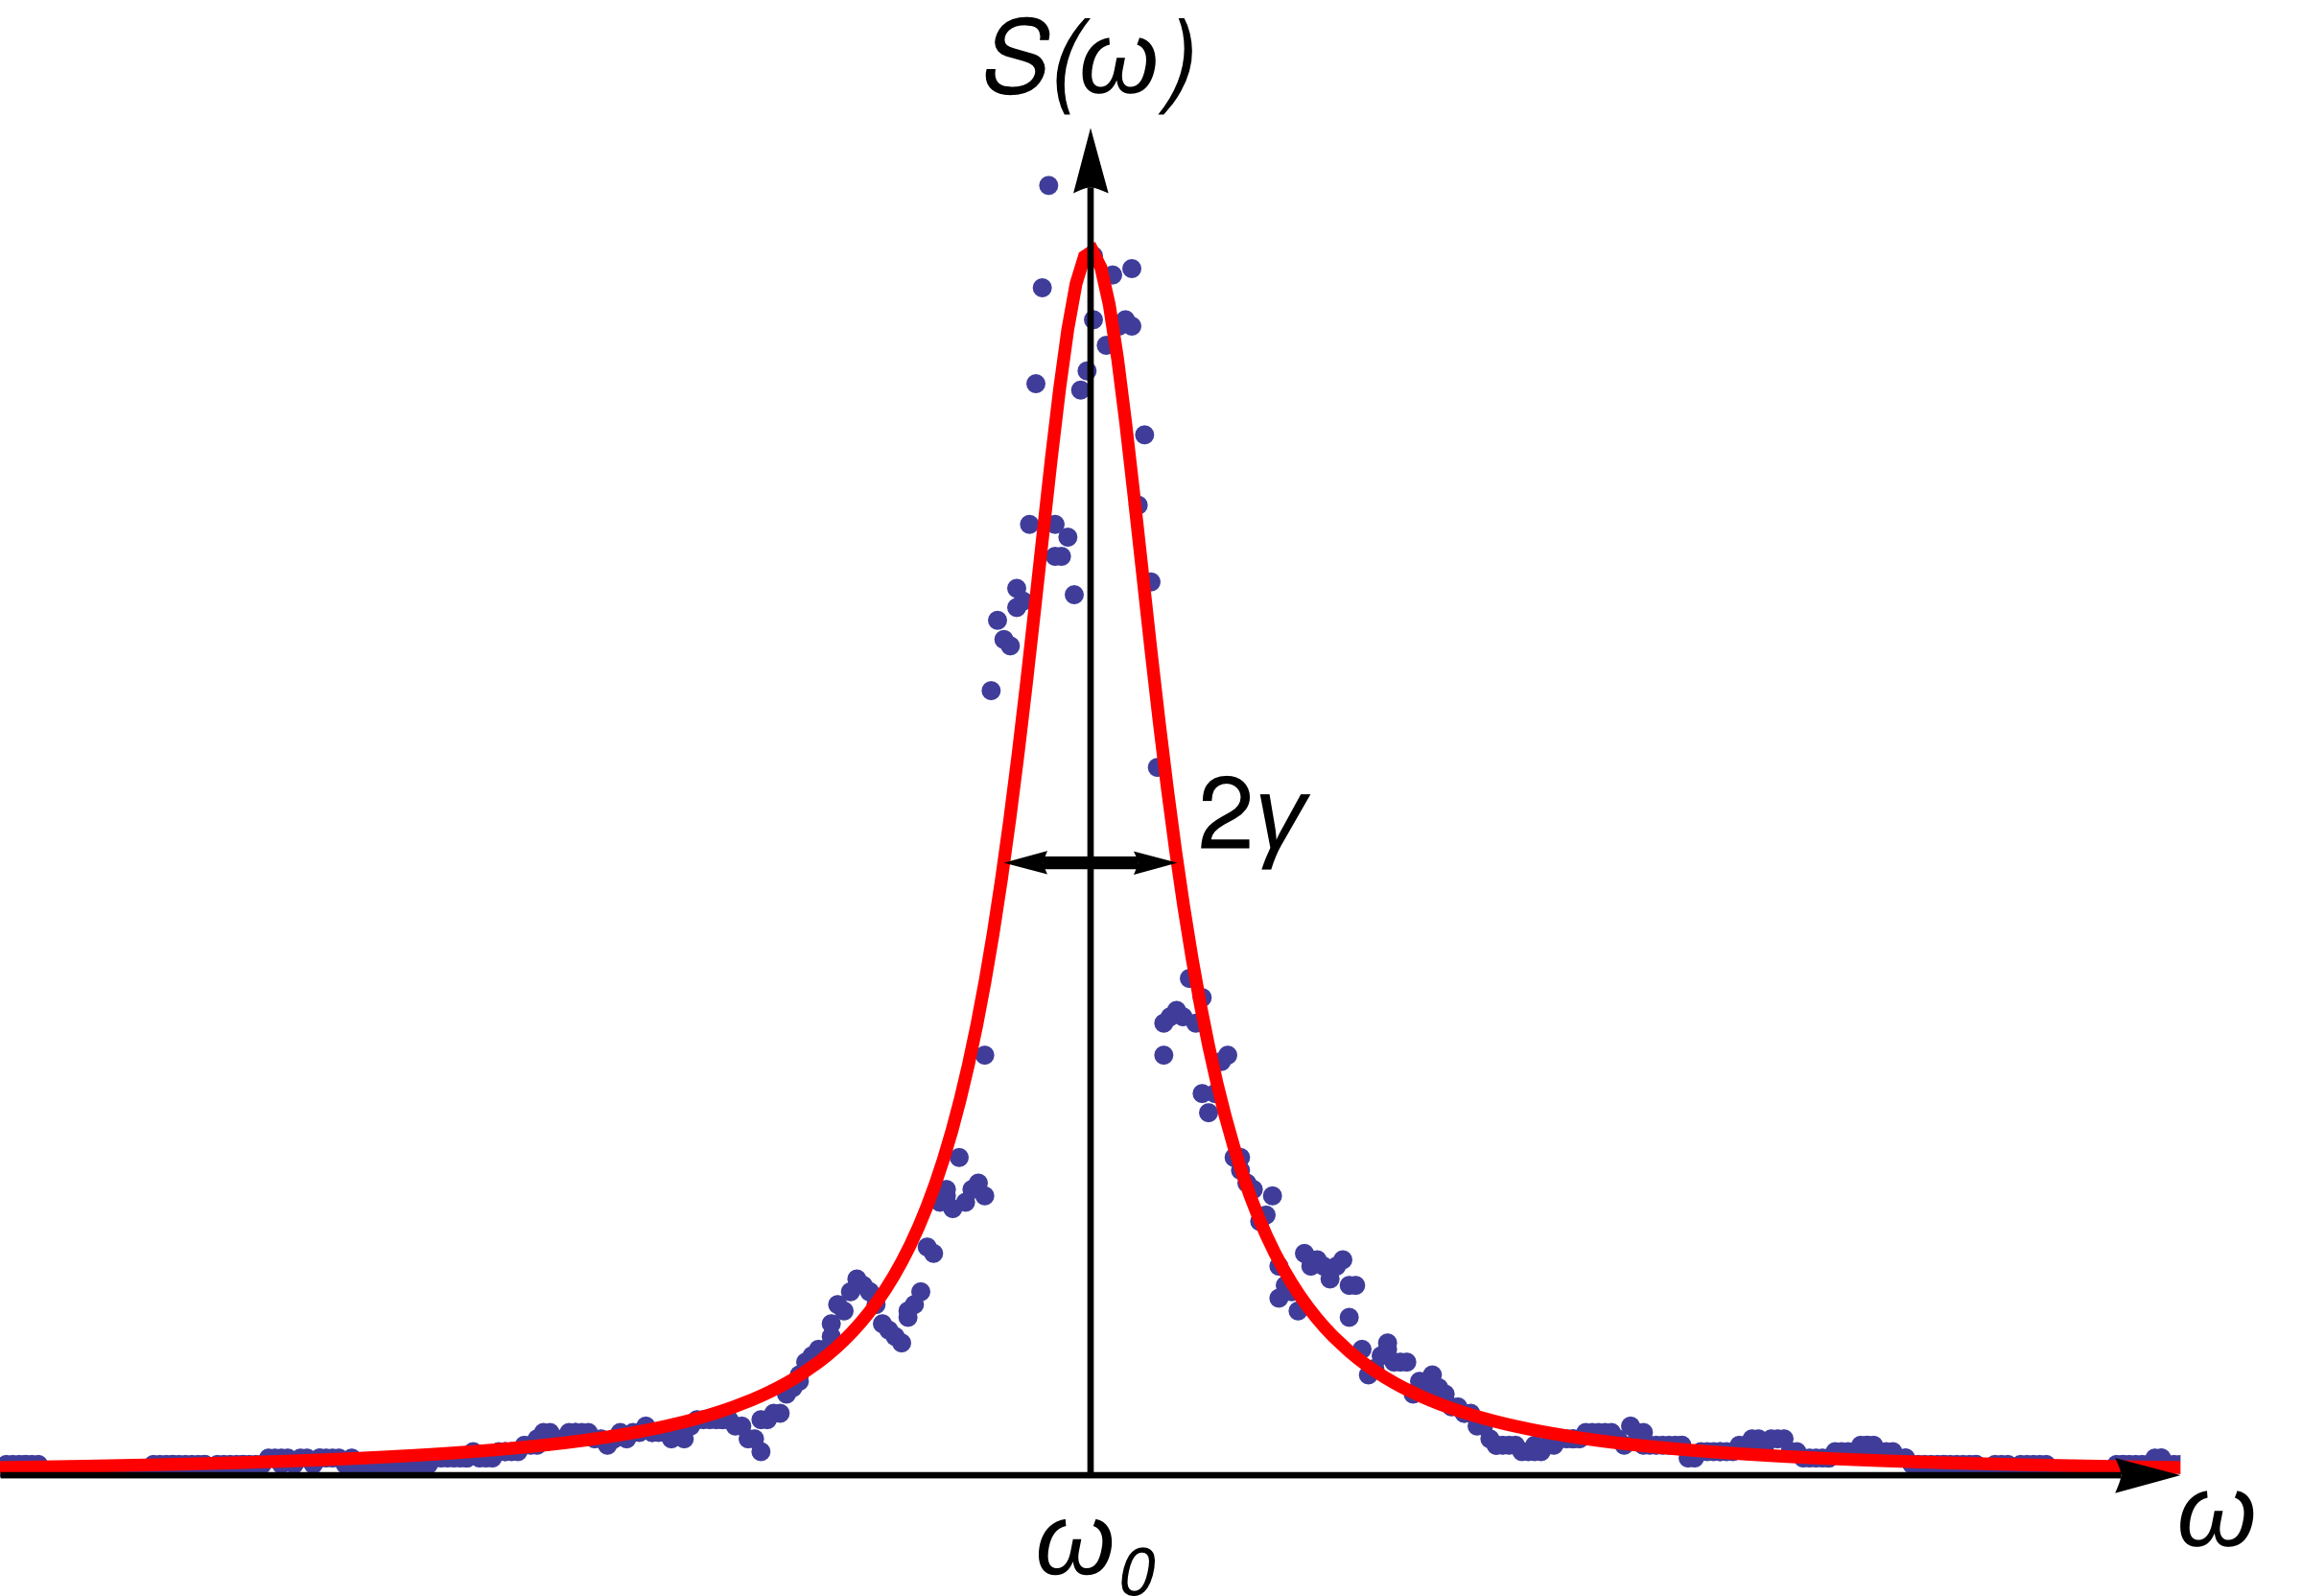
\includegraphics[width=6truecm]{slike/02_spekter.png}\qquad 
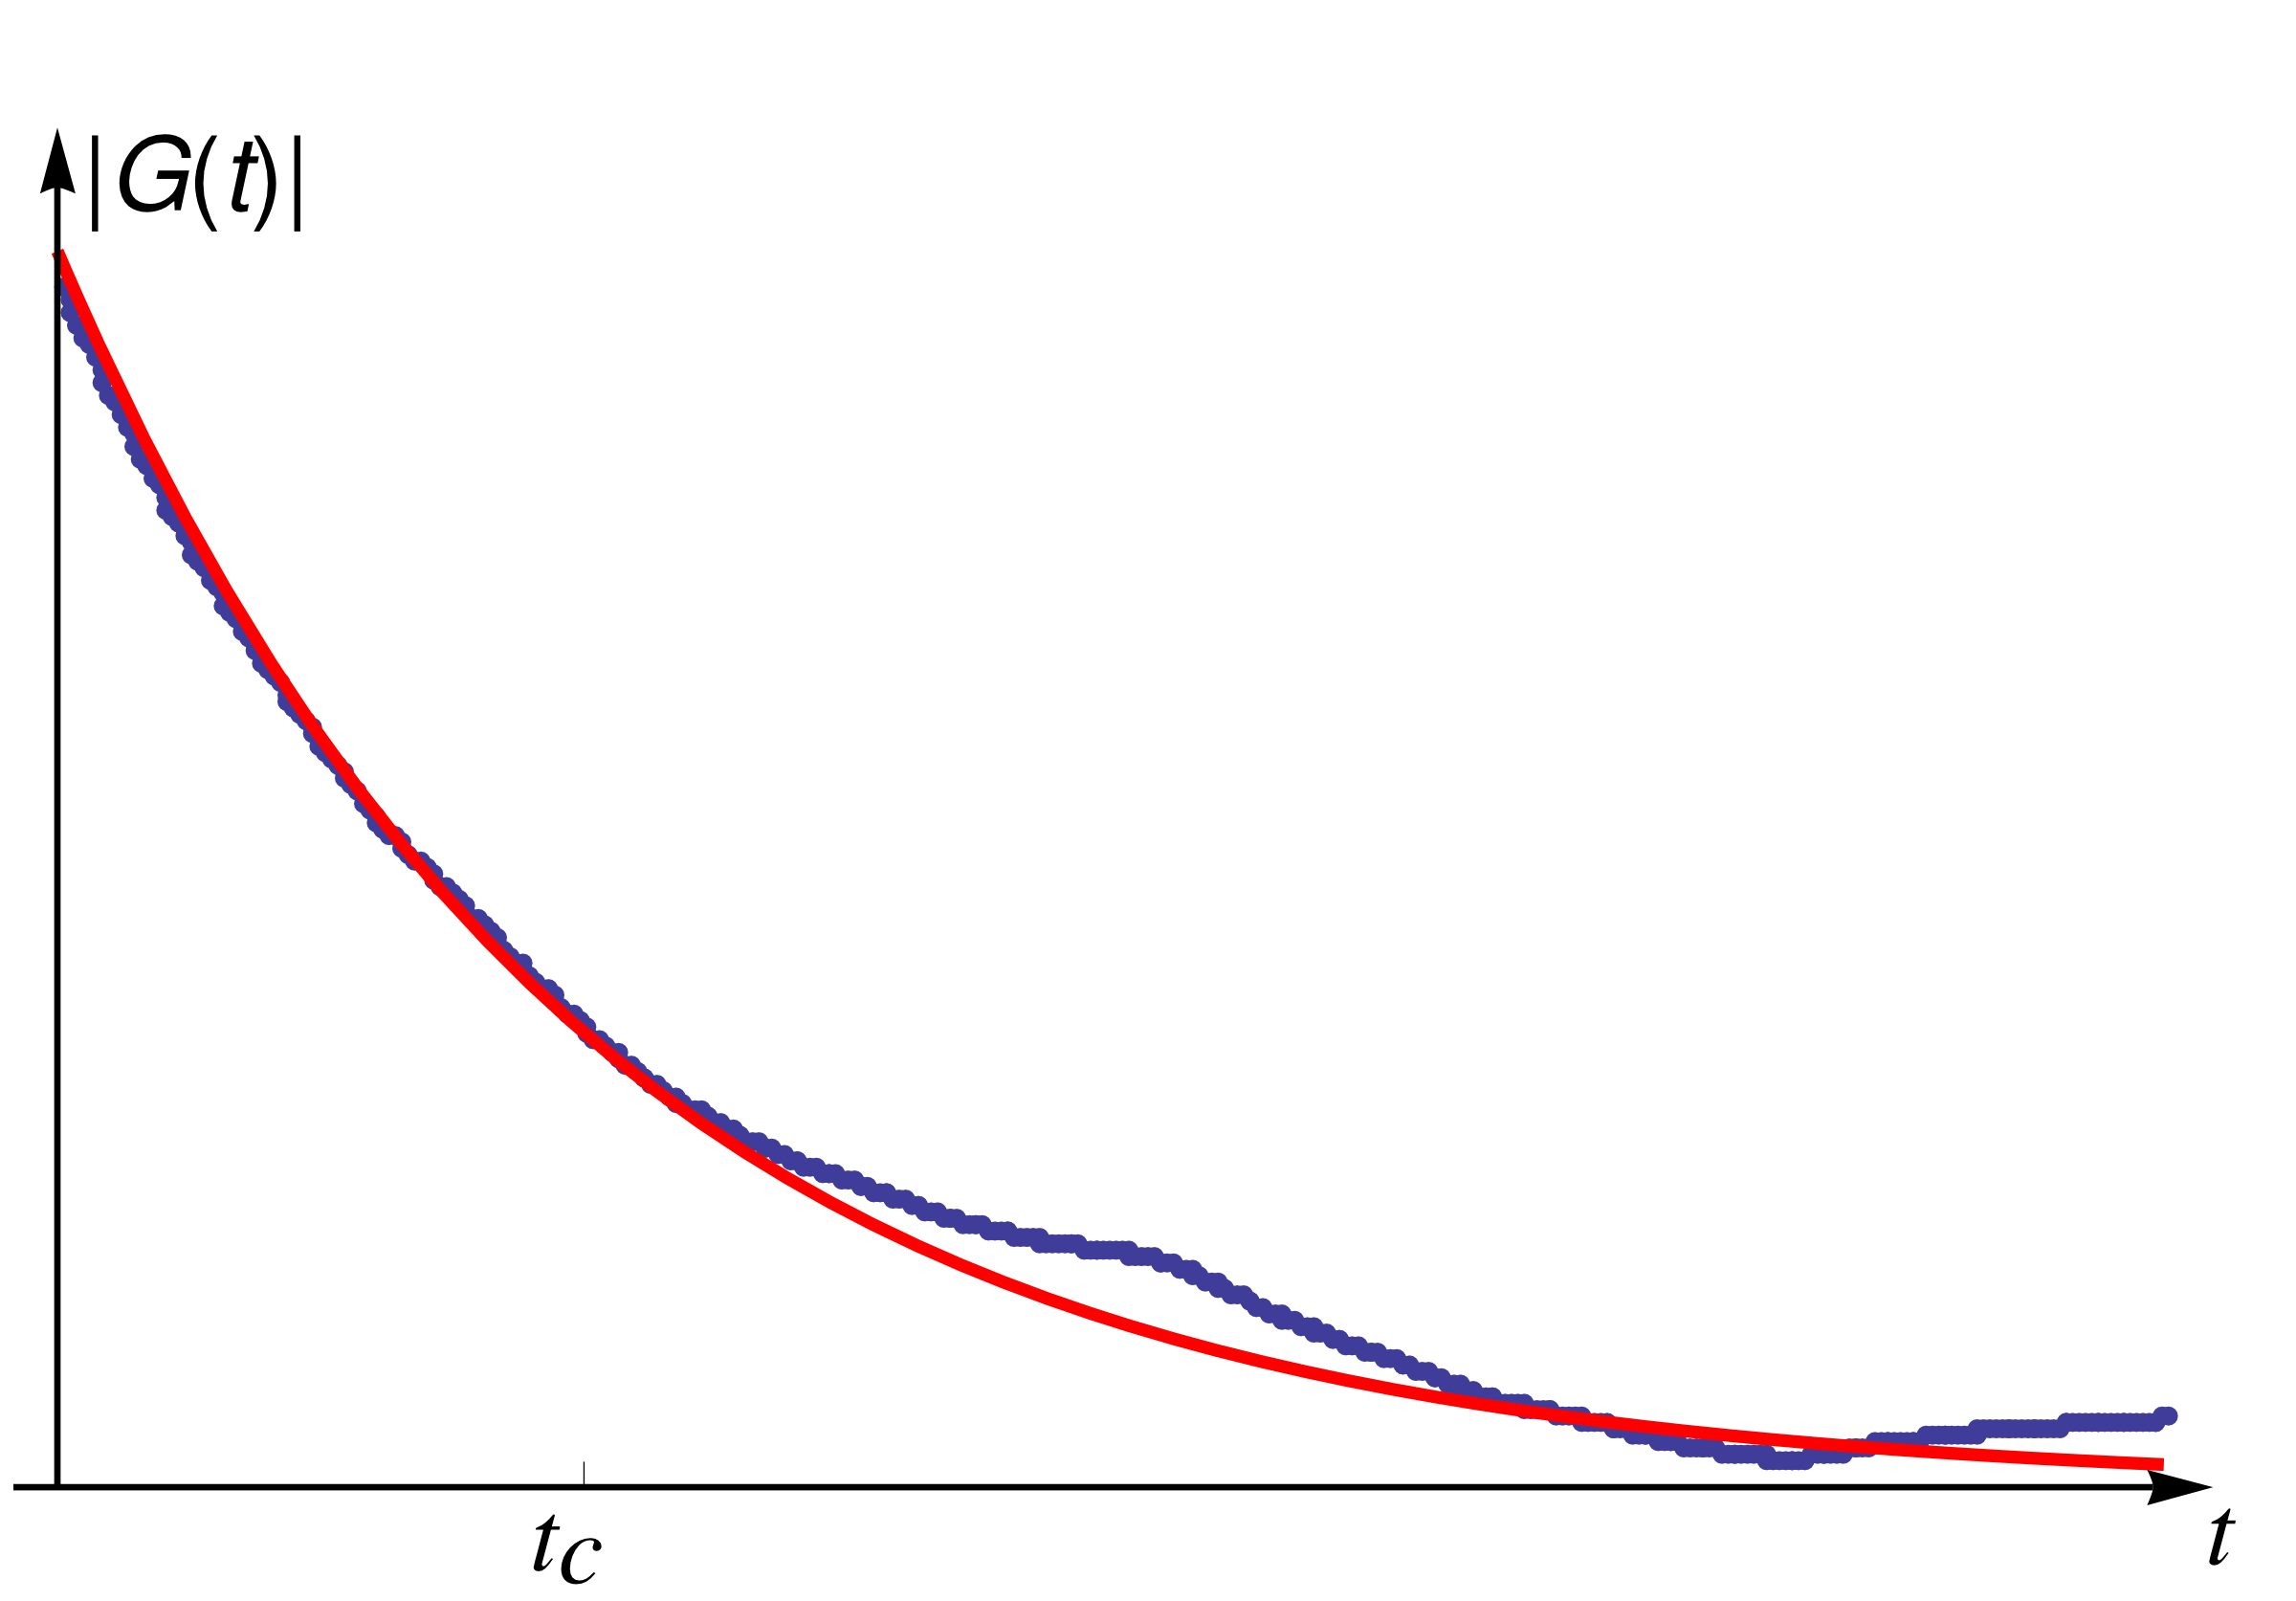
\includegraphics[width=6truecm]{slike/02_avtokorelacija.png}
\caption{Spekter in avtokorelacijska funkcija valovanja s slike~(\ref{fig:amplituda-intenziteta}).}
\label{fig:SpekterAc}
\end{figure}

\begin{definition}
\label{naloga-spekter}
Imejmo dve vrsti svetlobe. Prva naj ima avtokorelacijsko funkcijo, ki je eksponentno pojemajoča, druga
pa ima avtokorelacijsko funkcijo Gaussove oblike (enačbi~\ref{eq:gauss-eksponent}). Pokaži, da sta njuna
spektra oblike  
\begin{equation}
s(\omega)=
\frac{1}{\pi}\frac{\gamma}{(\omega-\omega_{0})^{2}+\gamma^{2}}, \quad \mathrm{in} \quad 
s(\omega)= \frac{1}{\sqrt{2}\pi\gamma}\exp\big(-
\frac{\left(\omega-\omega_{0}\right)^{2}}{2\pi\gamma^{2}}\big),
\end{equation}
kjer je $\gamma=1/t_{c}$ spektralna širina. 
\end{definition}

\noindent
Spektralne črte atomov so pogosto Lorentzove oblike, kar je posledica
eksponentnega razpada stanj (naravna širina). Dodatno se spektralne
črte razširijo zaradi trkov med atomi, vendar tudi to vodi do Lorentzove
oblike spektra. V plinih pa je pogostokrat prevladujoča razširitev črt
zaradi Dopplerjevega pojava. Spekter Dopplerjevo razširjene svetlobe
je, kot bomo videli kasneje, Gaussove oblike. V tem primeru iz enačbe~(\ref{eq:spekter-zveza})
sledi, da je tudi avtokorelacijska funkcija Gaussove oblike.\\

\begin{definition}\label{naloga-Planck}
Numerično pokaži, da je koherenčni čas svetlobe, ki jo oddaja črno telo s temperaturo $T$, približno enak
$t_{c}={\hbar}/{k_{B}T}$. Normaliziran spekter sevanja črnega telesa zapišemo 
kot \index{Planckov spekter}Planckov spekter 
\begin{equation}
s(\omega)=\frac{15}{\pi^{4}} \frac{\hbar^4\omega^3}{(kT)^4}/\left(e^{\hbar\omega/kT}-1\right)
\quad \textrm{za}~\omega >0,~\textrm{sicer}~s(\omega) = 0.
\label{eq:Planckov-spekter}
\end{equation}
\end{definition}

\begin{remark}{{\bf Fouriereva spektroskopija}}\\ \\
V prejšnjem razdelku smo videli, da časovno avtokorelacijsko funkcijo
merimo z Michelsonovim interferometrom. Dobljena povezava med
avtokorelacijo in spektrom je osnova za Fourierevo spektroskopijo,
ki ima nekatere pomembne prednosti pred drugimi metodami in se danes
precej uporablja, posebej v infrardečem področju.
\end{remark}


\section{Prostorska koherenca}
\label{Prostorska-koherenca}

\noindent
Vrnimo se k Youngovem poskusu\index{Youngov poskus} in obravnavi interference na dveh ozkih režah. 
Osvetljujmo zdaj reži s svetilom končnih razsežnosti. Svetilo naj še vedno sveti skoraj enobarvno
svetlobo in naj bo na simetrali med režama, kot kaže slika~(\ref{fig:shema-interferenca}).
\begin{figure}[h]
\centering
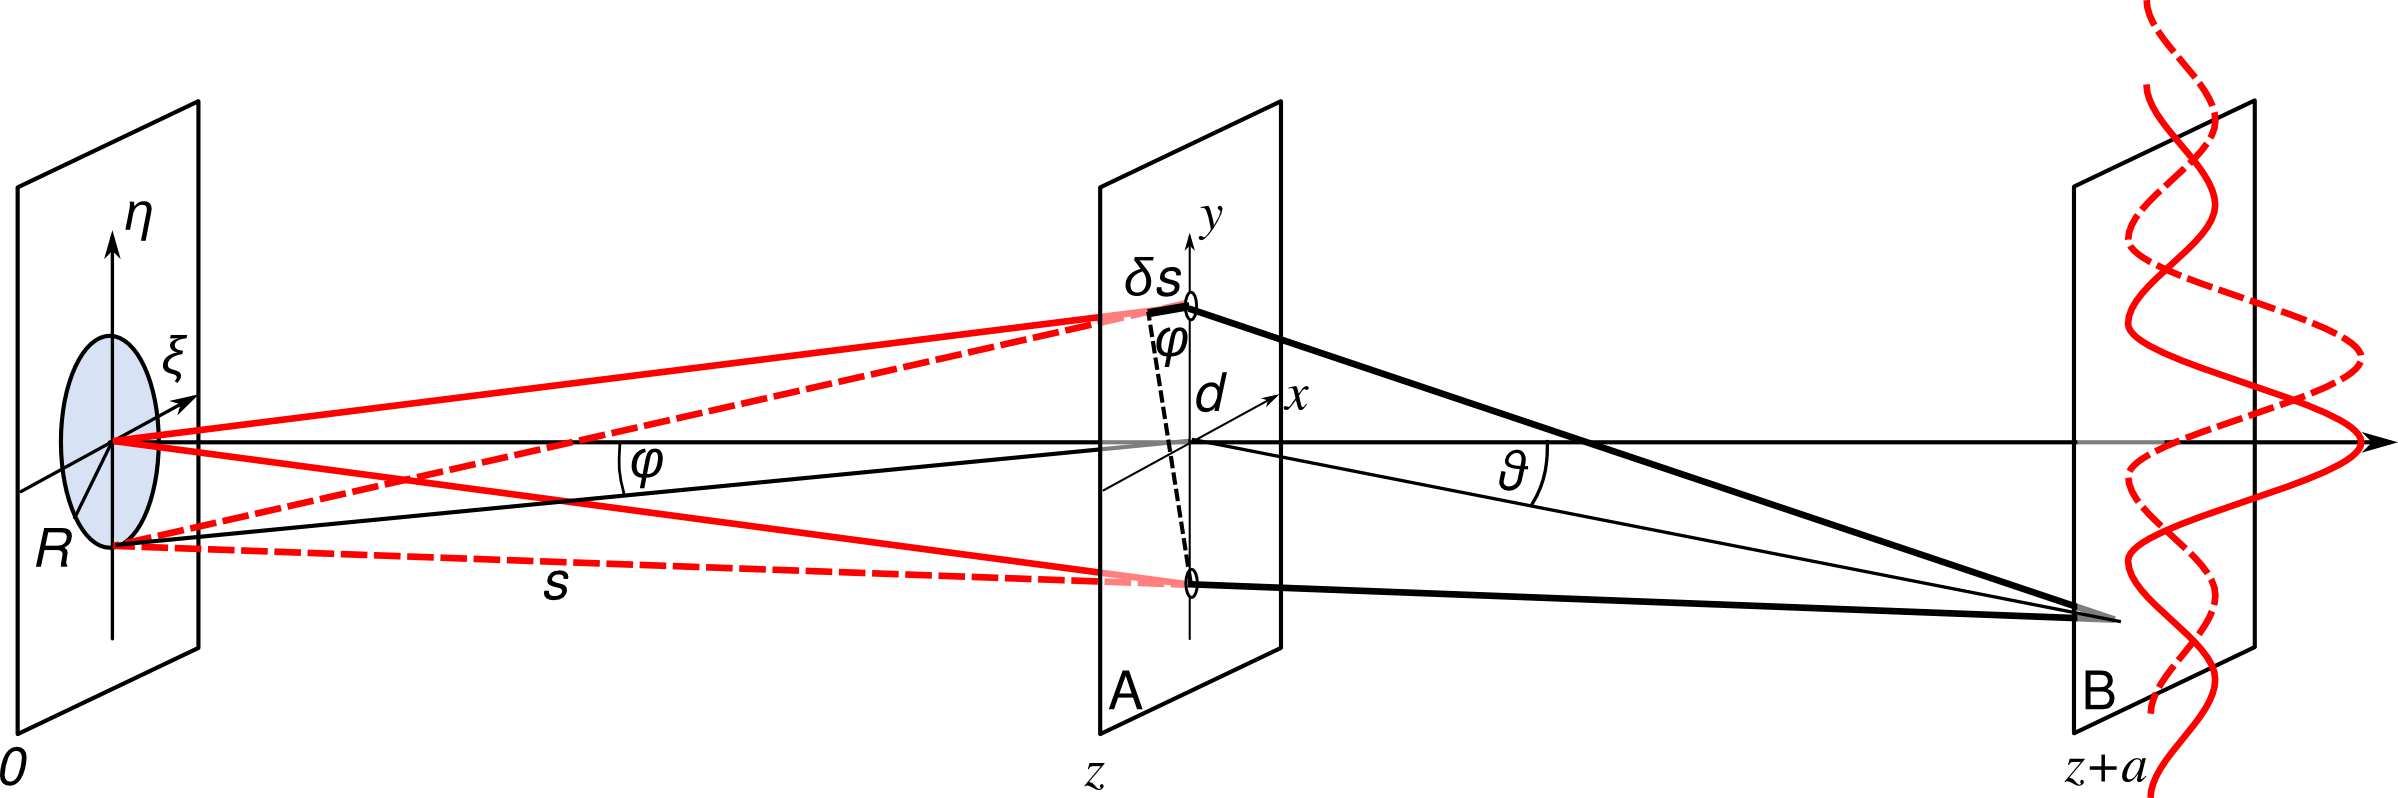
\includegraphics[width=14truecm]{slike/02_Diffraction_geometry.png}
\caption{Shema interferenčnega eksperimenta z razsežnim svetilom.
Svetilo velikosti $R$ postavimo v izhodišče koordinatnega sistema,
na zaslonu $B$ pa opazujemo sliko, ki nastane zaradi interference na dveh režah v
ravnini $A$. Zaradi končne dimenzije svetila so interferenčne proge,
ki jih tvorita robna žarka, premaknjene glede na proge centralnih
žarkov. Če je razlika poti za žarke z roba reda velikosti valovne
dolžine $\lambda$ ali več, se celotna interferenčna slika na zaslonu
$B$ izpovpreči.}
\label{fig:shema-interferenca}
\end{figure}
Žarka, ki izhajata iz sredine svetila (polna črta), 
opravita do rež v ravnini A enako dolgo pot in povzročita na zaslonu B 
interferenčne proge. Žarka, ki izhajata iz roba izvora (prekinjena črta), 
imata do rež različno dolgo pot, zato nastane med njima fazna razlika že do ravnine A, 
ki se prišteje fazni razliki do ravnine B. Interferenčne proge, ki jih tvorita 
robna žarka, so premaknjene glede na proge centralnih žarkov. Ker so žarki z roba
pri našem svetilu statistično neodvisni od žarkov iz sredine, z njimi
ne interferirajo. Celoten interferenčni vzorec je zato kar vsota interferenčnih
vzorcev žarkov iz različnih delov svetila. Če je razlika poti za žarke
z roba reda velikosti valovne dolžine $\lambda$ ali več, se celotna
interferenčna slika na zaslonu B izpovpreči. S slike razberemo, da
velja za razdaljo med režama $d$, pri kateri interferenčne proge
izginejo, približno 
\begin{equation}
\delta s\approx d\sin\varphi\approx d\frac{R}{z}\simeq\lambda\;\Rightarrow\;
d_{c}\simeq\frac{z\lambda}{R},\label{eq:prost_koh}
\end{equation}
kjer $d_{c}$ imenujmo prečno koherenčno razdaljo\index{Koherenčna razdalja}. Pogosto uporabljajo
tudi pojem \index{Koherenčna ploskev}koherenčne ploskve, to je območja, 
v katerem je fazna razlika v povprečju konstantna. Velikost te ploskve je približno $d_{c}^{2}$.
V območju koherenčne ploskve so tudi valovne fronte približno gladke.\\

\noindent
Zapišimo gornje ugotovitve nekoliko bolj natančno. Na zaslonu $B$
izmerimo gostoto svetlobnega toka, ki je sorazmerna povprečju kvadrata
električne poljske jakosti valovanj, ki izhajata iz obeh odprtin:
\begin{align}
\langle|E{}_{d}|^{2}\rangle & =\langle|K_{1}E_{1}+K_{2}E_{2}|^{2}\rangle\nonumber \\
&=  |K_{1}|^{2}\langle|E_{1}|^{2}\rangle+|K_{2}|^{2}\langle|E_{2}|^{2}\rangle+
2\Re K_{1}K_{2}^{*}\langle E_{1}(0)E_{2}^{*}(\tau)\rangle.
\end{align}
Pri tem je je $\tau=d\sin\vartheta/c$ zakasnitev valovanja iz druge odprtine
glede na valovanje iz prve. Faktorja $K_{1}$ in $K_{2}$ sta določena
z uklonom na posameznih odprtinah.
Interferenčna slika je vsebovana v podobnem členu kot pri Michelsonovem
interferometru, le da imamo v tem primeru namesto avtokorelacijske funkcije
navzkrižno korelacijsko funkcijo polj $E_{1}$ in $E_{2}$ iz obeh
odprtin.\\

\noindent
Kako je interferenčni člen povezan z lastnostmi svetila, brez težav
doženemo v izbranem primeru skoraj enobarvne svetlobe z osrednjo frekvenco
$\omega$. Tedaj lahko za zakasnitve $\tau$, ki so krajše
od koherenčnega časa, zapišemo 
\begin{equation}
E_{2}(\tau)=E_{2}(0)\, e^{-i\omega\tau}
\end{equation}
 in 
\begin{equation}
\langle E_{1}(0)E_{2}^{*}(\tau)\rangle=\langle E_{1}(0)E_{2}^{*}(0)\rangle 
e^{i\omega\tau}=J(P_{1},P_{2})\, e^{i\omega\tau}.
\end{equation}
Zadnji člen $\Re e^{i\omega\tau}= \cos(\omega \tau) = \cos(kd\sin\vartheta)$ da interferenčne
proge za koherentno osvetlitev zaslona $A$, povprečje produkta polj
v odprtinah ob istem času $J(P_{1},P_{2})=\langle E(P_{1},0)E^{*}(P_{2},0)\rangle$
pa meri stopnjo prečne koherence med obema odprtinama. Od velikosti
tega člena je odvisen kontrast interferenčnih prog. Izračunajmo ga.\\

\noindent
Polje v posamezni odprtini je vsota prispevkov iz celega izvora:
\begin{equation}
E(P_{j})=\frac{i}{\lambda}\int E(\xi,\eta)\frac{e^{iks_{j}}}{s_{j}}\, d\xi\, d\eta.
\end{equation}
Pri tem je $s_{j}$ razdalja med točko $(\xi,\eta)$ na izvoru in točko
$P_{j}=(x_{j},y_{j})$ na reži v ravnini A (glej sliko \ref{fig:shema-interferenca}).
Faktor pred integralom $i/\lambda$ smo dobili iz uklonske teorije.
Tako je 
\begin{equation}
J(P_{1},P_{2})=\frac{1}{\lambda^{2}}\int\int\langle E(\xi,\eta)E^{*}(\xi^{\prime},\eta^{\prime})\rangle\frac{e^{ik(s_{1}-s_{2}^{\prime})}}{s_{1}s_{2}^{\prime}}\, d\xi\, d\eta\, d\xi^{\prime}d\eta^{\prime}.\label{eq:field-correlation}
\end{equation}
V našem svetilu sevajo atomi neodvisno. Valovanji iz dveh točk svetila,
ki sta razmaknjeni za več kot $\lambda$, sta tako neodvisni in povprečje
njunega produkta je enako nič. Tako približno velja 
\begin{equation}
\langle E(\xi,\eta)E^{*}(\xi^{\prime},\eta^{\prime})\rangle=\lambda^{2}/\pi \cdot \delta(\xi-\xi^{\prime},\eta-\eta^{\prime})\langle|E(\xi,\eta)|^{2}\rangle.
\label{eq:delta-Zernike}
\end{equation}
Faktor $\lambda^{2}/\pi$ poskrbi za ustrezno normalizacijo. 
Naj bo oddaljenost svetila od zaslona $A$
mnogo večja od dimenzije svetila ($z\gg R$), tako da lahko imenovalec pod integralom
v izrazu~(\ref{eq:field-correlation}) nadomestimo z $z^{2}$ in postavimo
pred integral. Dobimo 
\begin{equation}
J(P_{1},P_{2})=\frac{1}{\pi z^{2}}\int\langle|E(\xi,\eta)|^{2}\rangle e^{ik(s_{1}-s_{2})}\, d\xi\, d\eta.\label{eq:Zernike1}
\end{equation}
Dobljeni izraz lahko še nekoliko poenostavimo, če razvijemo $s_{1}$
in $s_{2}$ do drugega reda: 
\begin{equation}
s_{j}=\sqrt{z^{2}+(x_{j}-\xi)^{2}+(y_{j}-\eta)^{2}}\simeq z+\frac{(x_{j}-\xi)^{2}+(y_{j}-\eta)^{2}}{2z},
\end{equation}
kjer sta $(x_{j},y_{j})$ koordinati točke $P_{j}$. Pišimo 
še $\langle|E(\xi,\eta)|^{2}\rangle=I(\xi,\eta)$, ki je do konstante natančno
enak intenziteti valovanja, ter $x_{2}-x_{1}=\Delta x$
in $y_{2}-y_{1}=\Delta y$. S tem dobimo znani rezultat, tako imenovani \index{van Cittert-Zernikov teorem}
van Cittert-Zernikov teorem\footnote{Nizozemski fizik Pieter Hendrik van Cittert, 1889--1959, in 
nizozemski fizik in nobelovec Frits Zernike, 1888--1966.}
\boxeq{eq:Zernike2}{
J(\Delta x,\Delta y)=\frac{e^{-i\phi}}{\pi z^{2}}\int I(\xi,\eta)e^{ik\frac{\Delta 
x\xi+\Delta y\eta}{z}}\, d\xi\, d\eta.
}

\noindent
Faza 
\begin{equation}
\phi=\frac{\pi}{\lambda z}[(x_{2}^{2}+y_{2}^{2})-(x_{1}^{2}+y_{1}^{2})]
\end{equation}
meri skupni premik interferenčnih prog, do katerega pride, kadar svetilo
ni na isti osi kot odprtini v zaslonu. Kadar ležijo svetilo in odprtini
v zaslonu $A$ simetrično na isti osi, je faza $\phi$ enaka nič.
Smiselno je vpeljati še normalizirano prečno prostorsko korelacijsko
funkcijo 
\begin{equation}
j(\Delta x,\Delta y)=\frac{J(\Delta x,\Delta y)}{J(0,0)}=\frac{e^{-i\phi}\int 
I(\xi,\eta)\exp\left[ik(\Delta x\xi+\Delta y\eta)/z\right]\, d\xi\, d\eta}
{\int I(\xi,\eta)\, d\xi\, d\eta}.
\label{eq:Zernike2-norm}
\end{equation}

\noindent
Dobljeni rezultat si je vredno nekoliko ogledati. Prečno prostorsko
korelacijsko funkcijo $J(P_{1},P_{2})$, ki določa kontrast interferenčnih
prog, smo izrazili kot 2-D  Fourierevo transformacijo intenzitete svetlobe
na samem svetilu (enačba \ref{eq:Zernike2}). Ob tem se spomnimo,
da velja podobna zveza med električno poljsko jakostjo v osvetljeni odprtini in njeno Fraunhoferjevo
uklonsko sliko, pri čemer so količine, ki nastopajo v obeh zvezah,
povsem različne. Različna je tudi veljavnost obeh: medtem ko je Fraunhoferjeva
uklonska formula veljavna le v veliki oddaljenosti, za bližje odprtine
pa je treba uporabiti Fresnelov izraz, je rezultat za $J(P_{1},P_{2})$
veljaven v obeh območjih.\\

\noindent
Ker je velikost svetila končna, $J(P_{1},P_{2})$ pri dovolj veliki
razdalji med točkama $P_{1}$ in $P_{2}$ gotovo pade na nič. Največja
razdalja, do katere je $J(P_{1},P_{2})$ še različna od nič, je ravno
prečna koherenčna razdalja $d_{c}$, ustrezna ploskev pa je koherenčna
ploskev $S_{c}$\index{Koherenčna ploskev}. Iz izraza za koherenčno razdaljo 
(enačba \ref{eq:prost_koh}) jo lahko ocenimo
\begin{equation}
S_{c}\simeq\frac{(\lambda z)^{2}}{S_{0}}\simeq\frac{\lambda^{2}}{\Omega_{0}},
\label{eq:koherencna-ploskev}
\end{equation}
kjer je $S_{0}$ površina svetila, $\Omega_{0}$ pa prostorski kot,
pod katerim je videti svetilo v ravnini $A$. \\

% \noindent
% Pri dovolj majhni razdalji med $P_{1}$ in $P_{2}$ je $J(P_{1},P_{2})$
% različen od nič. Postavimo kar limitni primer, ko je $P_{1}=P_{2}$, in 
% dobimo 
% \beq
% J(0,0)=\frac{1}{\pi z^{2}}\int I(\xi,\eta)\, d\xi\, d\eta,
% \eeq
% kar nam za velike $z$ predstavlja gostoto svetlobnega toka, ki vpada na zaslon $A$. 
% Z detektorjem velikosti $\sigma$ na zaslonu $A$ bi
% tako izmerili vpadno moč $J(0,0)\sigma=j\,S_0\sigma/z^{2}=j\, S_0\,\Omega_0$.
% \textcolor{red}{S tem smo upravičili izbiro normalizacijske konstante v 
% enačbi \ref{eq:delta-Zernike}. Faktorji 4 $\pi$? $\pi$? Ne razumem tega. }\\

\noindent
Oglejmo si primer. Naj bo svetilo v obliki kroga 
s polmerom $R$, obe odprtini v zaslonu naj imata koordinati $y$  enaki nič, razmik
med režama v smeri $x$ pa naj bo $d$. 
Za prečno korelacijsko funkcijo dobimo iz enačbe~(\ref{eq:Zernike2})
\begin{equation}
J(0,\Delta y)=2\frac{R^{2}I_{0}}{z^{2}}\,\frac{J_{1}(kRd/z)}{kRd/z}\;,
\end{equation}kjer je $J_{1}(x)$ Besselova funkcija. V ničlah Besslove funkcije
pade prečna korelacijska funkcija $J$ na nič in interferenčnega vzorca ne vidimo. 
Za prečno koherenčno razdaljo je zato smiselno vzeti ravno prvo ničlo, to
je pri
\boxeq{eq:okroglo_svetilo}{
d_{c}=3,83 \frac{z}{kR} = 0,61 \frac{\lambda z}{R}.
} \\

\noindent
Doslej smo obravnavali le valovanje v središču interferenčne slike na
zaslonu $B$, to je pri tako majhnih kotih $\vartheta$, da je zakasnitev
manjša od koherenčnega časa. Pri večjih kotih moramo upoštevati še
vpliv končnega koherenčnega časa, zaradi česar se kontrast interferenčnih
prog še dodatno zmanjšuje. \\

\noindent
Interferenčna slika na zaslonu $B$ je tako produkt časovnega in prostorskega
dela. V primeru dveh zelo tankih rež z razmikom $d$ dobimo na zaslonu
$B$ uklonske vrhove. Za nekaj različnih razmikov med odprtinama $d$ je intenziteta
svetlobe na zaslonu prikazana na sliki~(\ref{fig:Interferencna-slika}).
Če je $d\ll\lambda z/R$, je modulacija interferenčnih prog v sredini
popolna in se zaradi končnega koherenčnega časa zmanjšuje le pri večjih
kotih $\vartheta$. Pri nekaj večjem razmiku tudi v sredini kontrast
ni več popoln. Obenem se interferenčne proge zgostijo. Kadar je $d=3,83\,z/kR$,
dosežemo prvo ničlo Besselove funkcije $J_{1}(x)$ in interferenčni vzorec
prvič izgine. Takrat je razdalja med režama ravno enaka koherenčni razdalji valovanja.
Pri še večjih razmikih je Besselova funkcija negativna
in ponovno dobimo interferenčne proge, vendar so slabše izražene in z
nasprotno fazo, kar nam da v sredini temno progo. \\

\begin{figure}[h]
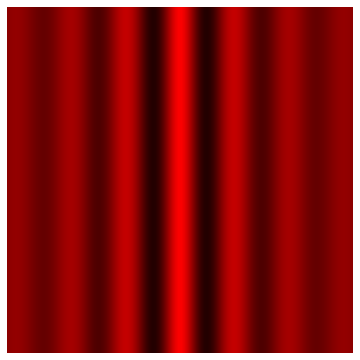
\includegraphics[width=0.24\textwidth]{slike/02_interferenca1.png}
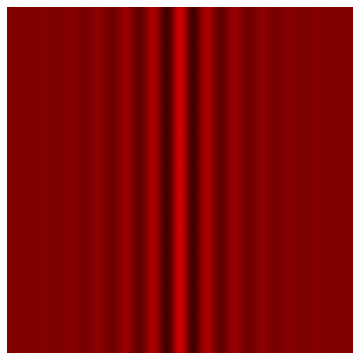
\includegraphics[width=0.24\textwidth]{slike/02_interferenca2.png}
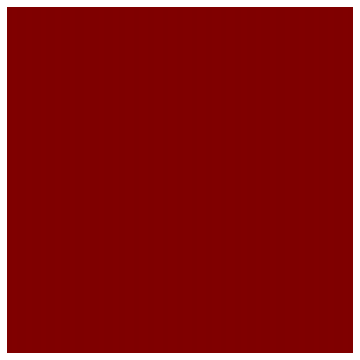
\includegraphics[width=0.24\textwidth]{slike/02_interferenca3.png}

\includegraphics[width=0.24\textwidth]{slike/02_interferenca4.png}
\caption{Interferenčna slika na zaslonu
$B$ za različne vrednosti razmikov med odprtinama $d = z/kR;\, 2z/kR;\, 3,832\,z/kR$ in $5,136\,z/kR$. 
Z večanjem razdalje med režama se proge zgostijo in kontrast se zmanjša. Koherenčni
čas svetlobe je $t_{c}=10/\omega$, kar še dodatno zmanjšuje modulacijo
interferenčnih prog. Pri $d=3,832\,z/kR$ dosežemo prvo ničlo Besselove
funkcije in interferenčni vzorec popolnoma izgine. Nato se interferenčne
proge zopet pojavijo, vendar z manjšim kontrastom in nasprotno fazo.}
\label{fig:Interferencna-slika}
\end{figure}

\begin{definition}
\label{naloga-cittert}
Svetloba s frekvenco $\omega$ in koherentnim časom $t_{c}$ izhaja
iz svetila s polmerom $R$ in vpada na zaslon, ki je $z$ oddaljen od svetila. 
V zaslonu sta dve zelo ozki reži na razmiku $d$. 
Pokaži, da je uklonska slika za zaslonom enaka
\begin{equation}
I/I_{0}=(1+2\,\frac{J_{1}(kRd/z)}{kRd/z}\cos(\omega\tau)e^{-\tau/t_{c}}),
\end{equation}
kjer je $\tau=d\sin\vartheta/c$ zakasnitev žarkov iz rež na zaslonu.
\end{definition}


\begin{remark}
Merjenje prečne koherenčne razdalje svetlobe
zvezd je osnova za Michelsonovo metodo določanja zvezdnih premerov.
Svetlobo izbrane zvezde zberejo v teleskop preko dveh manjših parov
zrcal, kjer sta zunanji zrcali na pomičnih rokah, tako da jih je mogoče
razmikati. Glavno zrcalo teleskopa zbere svetlobna snopa v goriščni
ravnini, kjer nastanejo interferenčne proge, če le pomični zrcali
nista preveč razmaknjeni. Iz razmika, pri katerem interferenčne proge
izginejo, je mogoče določiti premere bližnjih svetlih zvezd. Za zvezdo
s polmerom $10^{6}$ km v razdalji 5 svetlobnih let je prečna koherenčna
razdalja za zeleno svetlobo okoli $15$~m, kar je z Michelsonovim
zvezdnim interferometrom mogoče izmeriti. Pri zvezdah, ki so dlje
od nekaj deset svetlobnih let, metoda odpove.
\end{remark}
